%! Author = Админ
%! Date = 12.03.2022

% Preamble
\documentclass[11pt]{article}
% Packages
\usepackage{amsmath}
\usepackage{graphicx}
\usepackage{gensymb}
\usepackage{mathtools}
\graphicspath{{pictures/}}
% Document
\begin{document}
    \section{Problem}
    \begin{gather*}
        A(2,4,0); B(3,1,1); C(1,1,3); D(0,5,1)\\
        \overline{AB}(1,-3,1); \overline{CD}(-1,4,-2)\\
    \end{gather*}
    a) \newline % crossproduct of AB and CD gives you a normal vector ...
    \(M_1(x_1,y_1,z_1)\) lies on plane of AB \newline
    \(M_2(x_2,y_2,z_2)\) lies on plane of CD \newline
    Plane equation of AB: \newline
    \[\begin{bmatrix}
        x_1-2 & y_1-4 & z_1\\
        1     & -3    & 1  \\
        -1    & 4     & -2
    \end{bmatrix}=0 \]
    Plane equation of CD: \newline
    \[\begin{bmatrix}
          x_2-1 & y_2-1 & z_2-3\\
          -1    & 4     & -2   \\
          1     & -3    &  1
    \end{bmatrix}=0 \]
    . . .

    b) \newline
    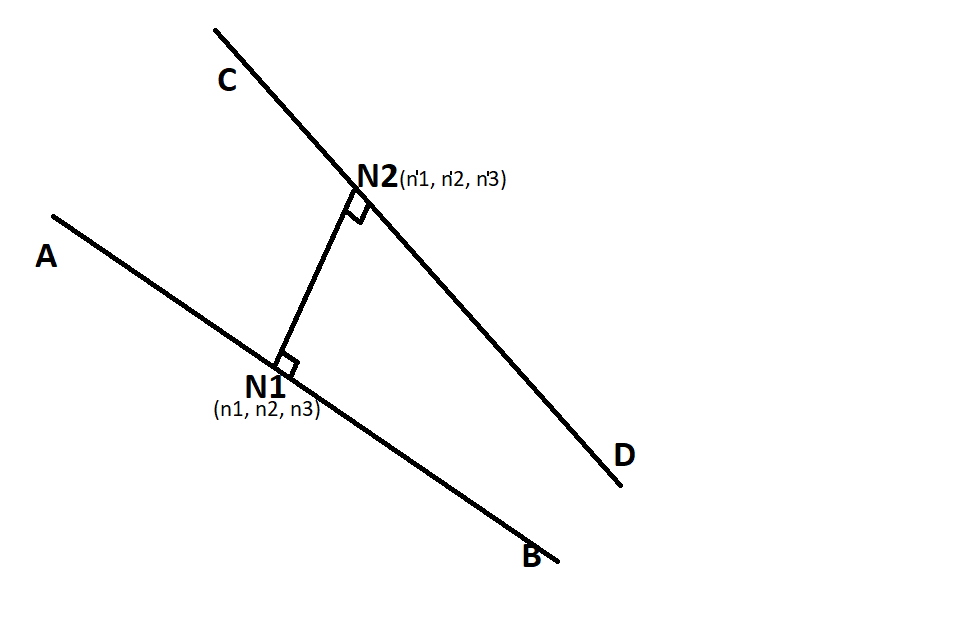
\includegraphics[width=200px]{taskOne.PNG} \newline
    1)
    \[\overline{AB}\cdot\overline{N}=0\]
    \[\begin{cases}
        x(t_1)=t_1+3   \\
        y(t_1)=-3t_1+1 \\
        z(t_1)=t_1+1   \\
    \end{cases}\]
    \begin{gather*}
        n_1=t_1+3\\
        n_2=-3t_1+1\\
        n_3=t_1+1\\
    \end{gather*}
    2)
    \[\overline{CD}\cdot\overline{N}=0\]
    \[\begin{cases}
          x(t_2)=-t_2    \\
          y(t_2)=4t_2+5  \\
          z(t_2)=-2t_2+1 \\
    \end{cases}\]
    \begin{gather*}
        n_1^\prime=-t_2\\
        n_2^\prime=4t_2+5\\
        n_3^\prime=-2t_2+1\\
        \overline{N_1N_2}(-t_2-t_1-3; 4t_2+6+3t_1; -2t_2-t_1)\\
    \end{gather*}
    \[\begin{cases}
          \overline{AB}\cdot\overline{N_1N_2}=0  \\
          \overline{CD}\cdot\overline{N_1N_2}=0  \\
    \end{cases}\]
    \[\begin{cases}
          7t_2+5t_1+6=0  \\
          5t_2+5t_1+7=0  \\
    \end{cases}\]
    \begin{gather*}
        t_1=0.5\\
        t_2\approx-2\\
        \overline{N_1N_2}(-1.5, -2.5, 3.5)\\
        \overline{|N_1N_2|}\approx4.5\\
    \end{gather*}


    \section{Problem}
    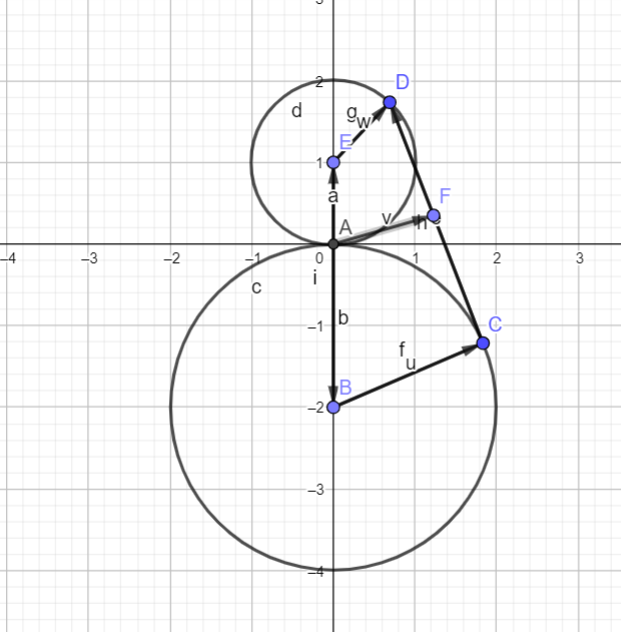
\includegraphics[width=200px]{coord3.PNG} \newline
    a) \newline
    \begin{gather*}
        \overline{AF}(t)-?\\
        \overline{AF}=\overline{AB}+\overline{BC}+\frac{\overline{CD}}{2}\\
        \overline{CD}=\overline{AE}+\overline{ED}-\overline{AB}-\overline{BC}\\
        \overline{AF}=\frac{\overline{AB}+\overline{BC}+\overline{AE}+\overline{ED}}{2}\\
        t_2=2t_1 \\
        \overline{AB}(0,2); \overline{BC}(2\sin{t}, -2+2\cos{t}); \overline{AE}(0, 1); \overline{ED}(\sin{2t}, 1-\cos{2t})\\
        \overline{AF}(2\sin{t}, \cos{t}+1-\frac{\cos{2t}}{2})\\
        x(t)=2\sin{t}\\
        y(t)=\cos{t}+1-\frac{\cos{2t}}{2})\\
    \end{gather*}



\end{document}